\documentclass[11pt]{article}
\usepackage[margin=1in]{geometry}
\usepackage{amsmath,amssymb,booktabs,microtype,graphicx,xcolor,longtable}
\usepackage[round]{natbib}
\usepackage[colorlinks=true,linkcolor=blue!50!black,urlcolor=blue!50!black,citecolor=blue!50!black]{hyperref}
\setlength{\parskip}{0.35em}\setlength{\parindent}{0em}
\title{\textbf{Dollar-Correct, Time-Wrong:\\
Twelve Backtest Bugs That Survive Reconciliation}}
\author{Charlie Yan\thanks{Draft v0.3 (journal-length), August 2026. Companion code:
\texttt{opentape}, an MIT-licensed library shipping every invariant below as a callable and
every bug class as a synthetic failing-then-passing test; no market data is required to
reproduce any exhibit in this paper. Every performance figure is labeled with its accounting
basis. Figures marked \textsc{invalid} are quoted \emph{as} invalidated examples, with the
corrected number alongside; none is a result of this paper.
Code, pre-registration documents and a data-availability statement: \url{https://github.com/charlieyanhx/backtest-bug-taxonomy}.}}
\date{August 2026}
\begin{document}\maketitle

\begin{abstract}
A backtest whose profit-and-loss reconciles to the cent can still be wrong by a factor of two
to eight in risk-adjusted terms---or can be measuring an exposure the strategy never claimed.
The defect in such cases lies not in the arithmetic of the dollars but in their \emph{timing},
their \emph{coverage}, the \emph{identity} of the instrument marked, the \emph{fills} assumed,
or the \emph{attribution} of the P\&L to the hypothesis under test. The standard defenses---reconciliation audits, multiple-
testing corrections, deflated Sharpe ratios, walk-forward protocols, leakage screens---do not
detect these failures, because every one of them takes the daily P\&L series as given. We
document twelve bug classes encountered in a single systematic options program, each with its
mechanism, the distortion it produced on live research, a
runtime-checkable invariant that prevents it, and a fully synthetic reproduction shipped as a
test. Two classes warrant emphasis. First, exit-day lumping---booking a multi-day trade's P\&L
on its exit date---inflates the Sharpe ratio \emph{only} when concurrent positions share
shocks: in simulation the exit-day-to-MTM Sharpe ratio climbs from 0.64 (purely
idiosyncratic P\&L, where lumping \emph{deflates}) to a plateau of 2.1--2.2 once shocks are
substantially shared---the same order of magnitude as, though slightly below, the
2.17--2.42$\times$ inflation observed in production, whose books carry sizing dispersion,
clustered entries and fat-tailed shocks the simulation omits. This explains why the bug survives toy
testing and why it is worst precisely for the correlated, stress-exposed books where accuracy
matters most. Second, \emph{attribution failure}---dollars, timing and coverage all correct
while the P\&L originates in an exposure the strategy was not testing---survives every check in
the other eleven classes; in our worked example a tape passing all of them earned its money
from a risk premium and a hedge path: constant-side controls on the identical entries scored
up to five times the signal's Sharpe---significantly better in paired form---while
side-randomized controls scored below zero in every one of 100 re-randomizations. We propose per-leg attribution plus a
side-randomized negative control as the minimum standard of evidence for any signal tape, and
we release the invariants as running code so that adoption costs an import rather than a
culture change.
\end{abstract}

\section{Introduction}
The quantitative research literature has developed an impressive apparatus for asking whether
a backtested result is \emph{statistically} credible. We can price the multiplicity of a
search \citep{hl, harvey2016}, deflate a Sharpe ratio for the number of trials that produced
it \citep{blp, blp2014b}, estimate the probability that an in-sample optimum is overfit
\citep{pbo}, embed the whole exercise in a protocol \citep{ahm}, and screen for the
train-test contamination that has produced a reproducibility crisis in machine-learning-based
science \citep{kn, reforms}. This apparatus shares a working premise: that the per-strategy performance number being
scrutinized was computed correctly in the first place. The premise is not universal---
\citet{ahm}'s protocol explicitly covers data and samples alongside economic motivation,
multiple testing, cross-validation, model dynamics, complexity and research culture---but that
category addresses data \emph{quality} and sample construction (survivorship, outliers,
selection) rather than the accounting mechanics by which a position file becomes a daily P\&L
series. It is those mechanics that concern us.

This paper is about the prior question. In building and auditing tapes for a systematic
options program---a documented research record spanning several months of intensive work over a
5.7-year data sample---the most damaging errors we encountered were not
statistical.
They were accounting errors: the dollars were right---reconciliations passed, totals tied to
the cent---but the dollars were placed on the wrong days, attributed to the wrong instrument,
computed over an incomplete calendar, or generated by an exposure the strategy never claimed to
test. Each produced a headline number that survived every statistical defense we could apply,
because those defenses operate on the daily series that the accounting error had already
corrupted.

We document twelve such classes (Table~\ref{tab:classes}), each with its mechanism, its
measured distortion on real research, a build-time invariant, and a synthetic reproduction that
lets a reader watch the bug appear and then be caught without access to our data or anyone
else's.

\textbf{We are explicit about what is and is not new here.} Most of the twelve are engineering
hygiene: known in principle to careful practitioners, absent from the published record chiefly
because nobody writes down what they fixed last quarter. Their value in this paper is
documentation and enforcement---measured magnitudes, and code that fails a build---not
discovery. Two of the twelve are different, and they are the paper's actual claims.

\textbf{Exit-day lumping is conditional, not universal} (\S\ref{sec:lump}). Booking each
trade's P\&L on its exit date, rather than marking it daily, leaves totals unchanged and is
widely known to distort risk statistics. What appears not to be known is \emph{when}: in our
simulations, under i.i.d.\ daily P\&L, lumping does not inflate the Sharpe ratio---it deflates
it (the magnitude of both effects is parameterization-dependent; \S\ref{sec:lump}). The
inflation requires that concurrent positions share shocks, because mark-to-market booking
concentrates a common shock onto one catastrophic day while exit-day booking disperses it
across the staggered exit dates of every trade that lived through it. Figure~\ref{fig:common}
traces the inflation ratio from 0.64 to its 2.1--2.2 plateau as commonality rises. The practical implication
is uncomfortable: the bug is invisible in the low-correlation test cases a developer is likely
to construct, and maximal in the correlated, stress-exposed books where the risk statistic
actually matters.

\textbf{Attribution failure survives everything else} (\S\ref{sec:attr}). A tape can pass
coverage assertions, reconciliation, sign checks, force-close discipline and calendar-time exit
location---and still be measuring a premium rather than a signal. Any structure with a nonzero
risk-premium or beta exposure harvests it whatever the overlay signal says; a roughly
side-symmetric signal then \emph{dilutes} the harvest instead of adding to it, and the
resulting Sharpe ratio is a diluted premium wearing the signal's name. The detection is cheap
and, in our experience, decisive: decompose the P\&L by leg, and re-run the identical tape with
randomized and constant sides. In the worked example of \S\ref{sec:attr} the constant-side
control scored 1.75 against the signal's 0.34.

Our contribution is deliberately unglamorous. It is a taxonomy, a set of assertions, and a
library. We argue that this is the right shape for the problem: statistical defenses are
applied by researchers who choose to apply them, whereas invariants run on every build. The
twelve classes below were each expensive to learn once; none should be expensive to learn
again.

\section{Related literature}\label{sec:lit}
\textbf{Selection and multiplicity.} \citet{lo2002} showed how sensitive the Sharpe ratio is
to the statistical properties of the return series it summarizes, and in particular to serial
correlation---an early instance of the general point that the \emph{shape} of the daily series,
not merely its mean and variance, drives the statistic. \citet{stw} formalized data-snooping
bias with the reality check; \citet{hl, harvey2016} brought multiple-testing discipline to the
cross-section of factors; \citet{blp2014b, blp} introduced the deflated Sharpe ratio and, with
\citet{pbo}, the probability of backtest overfitting. \citet{ahm} synthesize this line into a
practical protocol whose scope is broader than multiplicity alone, covering data and samples,
cross-validation, model dynamics and research culture. The centre of gravity of this line,
though, is \emph{how many} strategies were tried and how the winner's statistic should be
discounted; where it addresses data, it addresses sample integrity---survivorship, outliers,
selection---rather than whether the daily series under analysis was assembled correctly from
the positions that generated it.

\textbf{Return misdating and smoothed risk statistics.} \citet{glm} show that reported
returns on illiquid portfolios are a moving average of true returns, that this smoothing
understates volatility and inflates the Sharpe ratio, and that positive serial correlation in
reported returns is its signature; they supply a smoothing-adjusted Sharpe ratio as the
correction. Their source is stale pricing on assets that do not trade. Class~1 below is the
same bias arriving from a different door: the assets are perfectly liquid and continuously
priced, and the smoothing is introduced by an \emph{accounting convention}. We show in
\S\ref{sec:lump} that exit-day marking induces exactly the serial-correlation signature GLM
identify, and induces it precisely where it inflates --- which makes their diagnostic and their
correction directly applicable to a setting where nobody thinks to look for illiquidity,
because there is none.

\textbf{Practitioner pitfall catalogues.} Closest in spirit to this paper are the practitioner
catalogues of backtest sins: \citet{luo} on the ``seven sins'' of quantitative investing,
\citet{ldp10} on why machine-learning funds fail, and \citet{fldp} on honest backtest
reporting. Those catalogues name several of our classes in outline---look-ahead, survivorship-
style drops, cost fantasy---at the level of research practice and process. What they do not
contain is the accounting layer this paper supplies: measured distortion magnitudes from a live
program, the conditionality of class~1, the attribution control of class~12, and enforcement as
build-time code rather than checklist items. We position the twelve classes as the mechanized
layer beneath those checklists, not as their replacement.

\textbf{Leakage and reproducibility.} \citet{kn} document leakage as the dominant reproducibility
failure in machine-learning-based science and propose model-info sheets; \citet{reforms}
extends this to reporting standards. Leakage is adjacent to
our subject---both produce wrong numbers from clean intentions---and the boundary is not
perfectly clean: classes~8 and~10 are temporal leakage in \citet{kn}'s sense as well as
accounting defects (look-ahead selection on the exit; the signal embedded in the fill), and we
keep them in this taxonomy because the invariant that catches each is an accounting assertion
rather than a pipeline audit. The remaining classes are distinct from leakage: correct
information placed at the wrong time, on the wrong instrument, or credited to the wrong cause.

\textbf{Costs and implementability.} A parallel literature shows that anomalies survive
statistically and die economically: \citet{nvv} on transaction costs in the anomaly zoo,
\citet{fim} on trading costs at scale, \citet{cmp} on capacity. \citet{mp2016} document how
much published anomaly performance decays post-publication. Our class~5 (mid-fill fantasy) is
the accounting counterpart of this literature's economic point: the three-line convention we
propose (mid, friction-aware, full cross) makes the friction sensitivity of a result a
reported statistic rather than a discovered disappointment.

\textbf{Replication.} \citet{hxz} re-examine a large body of published results and find substantial
non-replication; \citet{clarge} bounds how much of the anomaly literature $p$-hacking alone
could explain.
Our classes suggest one under-explored contributor to non-replication: not that the original
authors searched too hard, but that the original tape mis-timed, mis-covered, or mis-attributed
its own P\&L in ways no reader could detect from a published table.

\textbf{Marking and valuation.} The accounting literature on fair-value measurement and the
practitioner literature on P\&L attribution both treat the timing of recognition as
first-order; the Basel-era P\&L attribution tests for internal models are, in effect, an
institutional version of the leg-decomposition we advocate in class~12. What is missing, and
what this paper supplies, is the translation of that discipline into research-stage backtests,
where no auditor is watching and the researcher's own reconciliation is the only gate.

\section{Setting and evidence standard}
All examples arise from one systematic SPY options program: hourly chain data spanning
2020--2026, short-premium and relative-value strategies, retail-to-mid-scale friction, holding
periods of days to weeks, and heavy position overlap during volatility episodes. The program's
standing evidence rules---each adopted after a specific failure---are: three fill lines (mid;
friction-aware; full cross, meaning buy at ask and sell at bid on every leg both ways, which is
the only go/no-go number); mark-to-market-daily marking padded to the full business calendar
with zeros on inactive days; a coverage line reported with every result (rows in, rows out, per
filter); pre-registered decision bars; and a test-count ledger.

Statistical conventions for every figure quoted in this paper: Sharpe ratios are
mean-over-standard-deviation of daily P\&L annualized by $\sqrt{252}$, computed on the
full-calendar series; confidence intervals are fixed-block bootstrap percentile intervals
\citep{kunsch} (2{,}000 draws, 21-trading-day blocks) unless stated otherwise; autocorrelations
are lag-1 sample correlations of the stated series.

We stress that none of the twelve classes is exotic. Each was found in code written by
competent researchers who were reconciling their numbers. That is the point: reconciliation is
a necessary check that is comprehensively insufficient.

\begin{table}[t]\centering\small
\footnotesize\setlength{\tabcolsep}{3.5pt}
\begin{tabular}{clll}\toprule
\# & Class & Measured distortion & Invariant \\ \midrule
1 & Exit-day lumping & Sharpe $\times$2.17--2.42 (conditional; \S\ref{sec:lump}) & one mark per held day \\
2 & Trajectory truncation & a ``12.6'' Sharpe, 100\% artifact & calendar-time exit location \\
3 & Boundary drops & 24\% of trades, non-randomly & tape count $=$ entry-log count \\
4 & Missing-leg deferral & 1.99 $\to$ 1.37; tail-day sign inverts & re-mark quote-less held days \\
5 & Mid-fill fantasy & ``8.58'' $\to$ $-8.20$ at real quotes & three lines; decide on full cross \\
6 & Active-day annualization & up to $\times$8 on sparse books & full-calendar padding \\
7 & Sign bug & net exceeds gross & assert Line 3 $\le$ Line 1 \\
8 & Dropped/retried candidates & revoked a live deployment & force-close, never drop \\
9 & Wrong-instrument lookup & P\&L sign flips (\S\ref{sec:short}) & exact-identity joins \\
10 & Same-snapshot execution & manufactures edge from pure noise & next-quote fills \\
11 & Calendar-indexed differencing & deletes every Monday & trading-day grid throughout \\
12 & \textbf{Attribution failure} & \textbf{signal 0.34 vs constant-side 1.75} & \textbf{leg decomposition + side control} \\
\bottomrule\end{tabular}
\caption{The twelve classes. Distortions are from live research in one program and are
illustrative magnitudes, not population estimates. All twelve have synthetic reproductions in
the companion library.}
\label{tab:classes}\end{table}

\section{Class 1: exit-day lumping, and when it actually bites}\label{sec:lump}
\textbf{Mechanism.} The whole trade's P\&L is booked on its exit day; days on which the
position was held and moving show zero.

\textbf{What it cost us.} A skew strategy quoted at 1.91 (exit-day basis, \textsc{invalid})
re-marked to 0.81; a premium sleeve 4.16 $\to$ 1.72; an aggregate book 4.78 $\to$
$\approx$2.2. Inflation of $2.36\times$, $2.42\times$ and $2.17\times$ respectively, with
totals unchanged in every case.

\textbf{The conditional result.} We simulate 120 overlapping ten-day trades on a 252-day
calendar, with each trade's daily P\&L a convex combination
$\rho \cdot (\text{common factor}) + (1-\rho) \cdot (\text{idiosyncratic})$, the common factor
carrying five planted crash days. (Full specification, from the checked-in script: common
factor $N(0.15, 1)$ daily with five crash days at $-12$; idiosyncratic $N(0.4, 1)$; unit
sizing; entry days uniform on the calendar; both series live on the same 252-day calendar with
zeros where nothing books; Sharpe as defined in \S3; median over 40 seeds per point.) Figure~\ref{fig:lumping} shows the canonical case
($\rho = 1$): identical cumulative totals, visibly different daily distributions---the exit-day
series simply does not contain the crash days, because each crash was dispersed across the
later exit dates of the trades that were open through it.
Figure~\ref{fig:common} varies $\rho$:
\begin{center}\small
\begin{tabular}{lccccccc}\toprule
$\rho$ (weight on common shock) & 0.0 & 0.2 & 0.4 & 0.5 & 0.6 & 0.8 & 1.0 \\
exit-day / MTM Sharpe ratio & 0.64 & 0.97 & 1.65 & 1.93 & 2.12 & 2.19 & 2.14 \\
\bottomrule\end{tabular}\end{center}
Under purely idiosyncratic P\&L, exit-day marking \emph{deflates} the Sharpe ratio; the
inflation appears only as positions come to share shocks, saturating near 2.1--2.2$\times$.
That is the right order of magnitude for the $2.36\times$, $2.42\times$ and $2.17\times$
measured in production---and slightly \emph{below} the two larger ones, which we state plainly:
the simulation reproduces the mechanism, not the full production magnitude. Sizing dispersion,
clustered entries and fatter-than-Gaussian shocks are all present in the production book and
all absent from the simulation, and each pushes the ratio higher.

\textbf{The mechanism is portfolio-level smoothing, and it leaves GLM's fingerprint.} At the
level of a single trade, exit-day marking \emph{concentrates}: eleven days of P\&L collapse onto
one. At the level of the portfolio it \emph{smooths}, because a shock common to many open
positions is dispersed across their staggered exit dates. That is the same operation
\citet{glm} model for illiquid holdings, and it leaves the same trace. In the simulation, the
first-order autocorrelation of the exit-day series rises monotonically with commonality ---
$+0.02$ at $\rho=0$, $+0.21$ at $\rho=0.5$, $+0.29$ at $\rho=1$ --- rising as the inflation
rises to its plateau (the plateau itself is flat within seed noise). The MTM-daily series
moves the other way, from $+0.16$ at $\rho=0$ to $-0.03$
at $\rho=1$.

\textbf{That second series is the important one, and it disciplines the diagnostic.} A
\emph{correctly} marked daily series is not serially uncorrelated: with overlapping multi-day
holds, consecutive days share open positions, and the resulting variation in inventory induces
positive autocorrelation --- here $+0.16$ --- with no marking error whatsoever. So the naive
reading, that positive serial correlation in a liquid-instrument P\&L series indicates a marking
convention, is wrong: it would flag every correctly marked book with overlapping holds. What
separates the two is the \emph{sign of the relationship with commonality}, not the level.
Correct marking's autocorrelation is an overlap artifact that common shocks wash out, so it
\emph{falls} as positions correlate; lumping's is manufactured by the convention itself, so it
\emph{rises}. The usable test is therefore conditional: estimate the autocorrelation the
position overlap alone implies, and treat only the excess --- and specifically excess that grows
with cross-position correlation --- as evidence of a marking convention. Where that test fires,
GLM's smoothing-adjusted Sharpe is the right correction to apply. We flag this as a diagnostic
worth developing rather than a validated instrument: we have calibrated it on a simulation and
one book, and its false-positive rate on a wider sample of correctly marked, overlapping-hold
strategies is unmeasured.

\textbf{Why this matters beyond bookkeeping.} A developer testing a marking convention on
synthetic i.i.d.\ P\&L will conclude the convention is harmless. The convention is harmless
\emph{there}. It is maximally harmful for short-volatility, correlated, episode-clustered books
---the books whose risk statistics are most consequential and most scrutinized. We know of no
prior statement of this conditionality.

\textbf{Invariant.} One mark row per trade per held trading day, asserted at build time. The
assertion is cheap because marks telescope: interior re-marks cannot change a trade's total, so
enforcing coverage cannot alter reconciled dollars---only their timing.

\begin{figure}[t]\centering
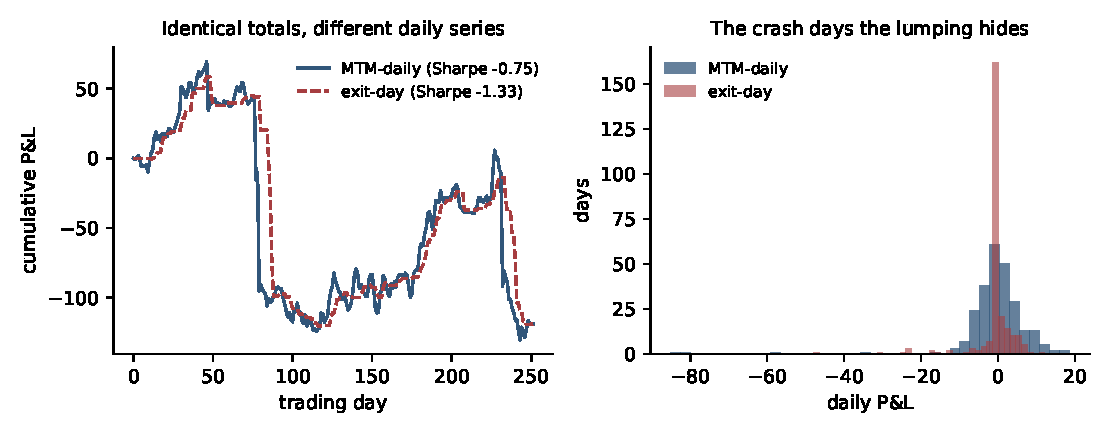
\includegraphics[width=\textwidth]{fig_p1_lumping.pdf}
\caption{Synthetic 120-trade book, fully common shocks. Left: cumulative P\&L is
identical by construction; the daily paths are not. Right: the exit-day series is missing the
crash days entirely---they have been smeared across later exit dates.}
\label{fig:lumping}\end{figure}
\begin{figure}[t]\centering
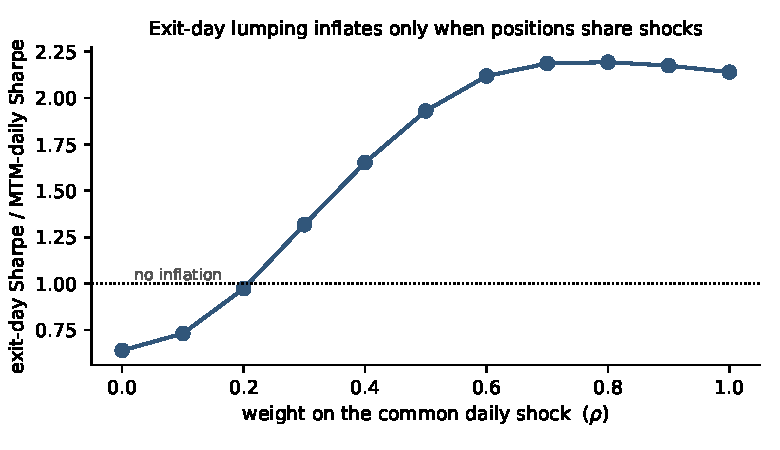
\includegraphics[width=0.68\textwidth]{fig_p1_commonality.pdf}
\caption{The inflation is conditional on shock commonality. At $\rho=0$ exit-day
marking deflates the Sharpe ratio (0.64$\times$); at $\rho=1$ it inflates it (2.14$\times$).
Median over 40 seeds per point.}
\label{fig:common}\end{figure}

\section{Classes 2--11: the catalogue}\label{sec:short}
\textbf{Class 2, trajectory truncation.} The exit is located by \emph{index} into a per-trade
trajectory array. When a leg leaves the quoted panel mid-hold---delisting, a moneyness filter,
or quote loss, all of which concentrate on stress days---the index silently reads a stale row.
Cost: a ``12.64'' Sharpe (\textsc{invalid}) that was 100\% artifact, and a second strategy's
4.14 that died on the same re-audit. Invariant: locate exits on the calendar and force-close a
leg that leaves the panel at its last real quote.

\textbf{Class 3, boundary drops.} Splitting a tape into periods drops trades straddling a
boundary. The drop is not random---it selects long and escalating holds, i.e.\ the
risk-carrying trades. Cost: a walk-forward missing 24\% of its trades. Invariant: per-period
tape count equals entry-log count.

\textbf{Class 4, missing-leg deferral.} Per-leg marks are written only on days the leg has a
quote; deep in-the-money legs lose quotes on crash days, so the crash-day move lumps onto the
next quoted day. Totals unchanged, tail-day \emph{timing inverts}: the book can print a gain on
the crash day. Cost: a core sleeve 1.99 $\to$ 1.37. Caught only when someone asked why a
short-volatility book's \emph{best} day was a crash day---which we now run as a standing
diagnostic. Invariant: re-mark quote-less held days (carry plus intrinsic shift, floored at
intrinsic: model-free and total-preserving) and assert coverage.

\textbf{Class 5, mid-fill fantasy.} One accounting line, at mid or at modeled fills. Cost: an
``8.58'' (modeled, \textsc{invalid}) that was $-8.20$ at real crossed quotes and reached a live
deployment before the three-line rule existed; separately, a $+9.67$ at mid that was $-14.6$ at
1\% friction. Invariant: three lines always, decide on full cross, and report the
line-1-minus-line 3 gap as the result's friction sensitivity.

\textbf{Class 6, active-day annualization.} Computing the Sharpe ratio over active days only
and annualizing by $\sqrt{252}$. Cost: up to 8$\times$ on sparse books; one $+15.97$
(\textsc{invalid}; full-calendar re-mark $+1.98$---the source of the 8$\times$). Invariant: pad
to the full calendar with zeros.

\textbf{Class 7, sign bug.} Net exceeding gross---the spread credited rather than paid---via
sign conventions in multi-leg friction. Invariant: assert Line 3 $\le$ Line 1 every run.

\textbf{Class 8, dropped or retried candidates.} Entries that never resolved in-window quietly
discarded, or retried until they resolve favorably: look-ahead selection on the exit. Cost:
revoked a live deployment (honest Sharpe $\approx 0$ from ``8.04'', \textsc{invalid}).
Invariant: force-close, never drop; class~3's count check catches the residue.

\textbf{Class 9, wrong-instrument lookup.} Forward P\&L looked up by bucket (delta band,
moneyness bin) rather than exact contract; as the underlying moves, the bucket re-maps to a
different instrument and the ``position'' silently mutates. Our synthetic reproduction is
deliberately stark: with two strikes and one day of spot movement, the bucket join reports
$-0.40$ and the exact-identity join $+1.50$ on what is nominally the same trade. Invariant:
join on exact (expiration, strike, type).

\textbf{Class 10, same-snapshot execution.} Filling at the quote that generated the signal. For
any quote-derived signal this embeds the signal in the fill. In the reproduction, a ``buy the
dip'' rule applied to pure i.i.d.\ quote noise earns a large apparent edge when filled at the
signal quote and exactly zero when filled at the next one. Invariant: next-quote fills,
strictly after signal time.

\textbf{Class 11, calendar-indexed differencing.} Differencing on a calendar-date index deletes
every Monday and post-holiday observation, or lets a hold specified as ``two days'' silently
span a weekend---four calendar days of exposure booked as two. Invariant: all differencing and
holding periods on the trading-day grid.

\section{Class 12: attribution failure}\label{sec:attr}
\textbf{Mechanism.} Dollars right, timing right, coverage right, fills honest---and the P\&L
still does not come from the hypothesis. Any structure carrying a risk premium or a beta
harvests it regardless of the overlay signal. If the signal is roughly side-symmetric, it
splits the book between premium-collecting and premium-paying trades, and the net result is a
\emph{diluted premium} that the researcher reads as a signal result.

\textbf{Worked example} (all figures full cross fills, marked daily, full calendar,
2020-09 to 2026-05). A residual-fade tape passed every check in classes 1--11: coverage
asserted, counts tied, sign check held, force-close applied, calendar-time exits. Headline:
Sharpe 0.34, 95\% CI $[-0.18, 0.90]$. Three diagnostics then located the money:
\begin{itemize}\itemsep0.05em
\item \textbf{Concentration.} 98\% of the P\&L came from a single calendar year; another year
lost roughly a third of the total.
\item \textbf{Leg decomposition.} In the profitable year the \emph{option leg lost} money while
the delta hedge made it---i.e.\ the tape's P\&L was a hedge path, not an option-selection
result.
\item \textbf{Side-randomized control.} Re-running the identical entries with the side
replaced: signal 0.34, random sides mean $-1.57$ over 100 re-randomizations (SD 0.39, 95\%
range $[-2.28, -0.84]$, every seed negative---quote the distribution, never one draw),
\textbf{always-short 1.75} $[0.69, 3.32]$,
always-long $-2.28$. The strategy's own structure, stripped of its signal, scored five times
better than the signal. The single-arm intervals overlap---always-short
$[0.69, 3.32]$ against the signal's $[-0.18, 0.90]$---so the decisive comparison is paired:
on the identical calendar the daily difference (signal minus always-short) has Newey--West
$t = -3.62$ and is negative in all seven calendar years. The signal is significantly
\emph{worse} than its own structure.
\end{itemize}
The signal's genuine discrimination was approximately \$4.9 per trade against a short-side
premium of roughly \$24 per trade: real, and roughly five-fold too small to matter. No
accounting audit could have reached this conclusion, because no accounting was wrong.

\textbf{Invariant (two-part).} (i) Decompose P\&L by leg and require the thesis leg to carry
the result. (ii) Re-run the identical tape with randomized and constant sides; if a constant
side beats the signal by more than the paired comparison's sampling error, the signal is not
what carries the tape. Both are inexpensive---the second is a loop over the
existing tape with one array replaced---and in our experience neither is standard practice.
Two cautions bound the claim. The controls assume a roughly side-symmetric signal, and the leg
split assumes a decomposition that reflects the thesis: for delta-hedged books the
option-versus-hedge split is convention-dependent, and a genuine volatility signal can
legitimately show hedge-leg profits in a trending year. Like the class-1 autocorrelation
diagnostic, we therefore flag the pair's false-positive rate on correctly attributed
strategies as unmeasured---a standard worth developing, not a validated instrument.

\section{Two audits that passed and were still wrong}
\textbf{Case A.} A competent pre-deployment leakage audit produced eight severity-ranked
findings, correctly identified a real exit-fill leak worth $-1.41$ Sharpe in isolation
(8.04 $\to$ 6.63 on that strategy's all-sample basis), corrected the headline to 6.81
all-sample and 6.10 out-of-sample once all fixes were combined---the entry-side fix added back
$+0.30$---(that strategy's own basis, later
\textsc{invalid} in full), and certified the strategy operational. It was subsequently
invalidated entirely by classes 1 and 8. The audit was not incompetent; it was scoped to check
the tape against itself, and both defects lived upstream of the tape it was given.

\textbf{Case B.} A five-year projection turning \$250k into \$18.5M (Sharpe ``6.7'',
\textsc{invalid}) rested on a slippage constant of \$4.80 per contract that had never been
measured. The measured value was \$9.68. At the measured value the strategy loses money at
full-spread fills. This is class~5 with an unvalidated parameter in the friction-aware line: a
single number, never checked, propagating through an otherwise careful analysis.

\textbf{The lesson.} Audits validate computations; invariants constrain constructions. An audit
runs when someone schedules it, examines what it is pointed at, and cannot see the assumptions
baked into its inputs. An invariant runs on every build and fails loudly. The twelve classes
argue for shifting effort from the former to the latter.

\section{What a screen can and cannot tell you}
The class-12 example carries a final lesson worth separating out. The screen that motivated
that tape projected approximately \$2.75 per contract net; the tape realized \$2.56---the
screen's \emph{mean} was accurate to within 7\%. What the screen could not see was everything
that determined whether the strategy was worth running: the concentration of P\&L in one year,
the 56\% of gross consumed by the spread, the commissions taking half of the remainder, and the
daily volatility that set the Sharpe ratio at 0.34.

Screens are accurate about means and uninformative about risk. The dangerous ones are precisely
those validated on average P\&L per trade, where concentration and volatility are structurally
invisible. We suggest that any screen used to justify building a tape should be reported with
the explicit caveat that it constrains the mean only---and that the tape, not the screen, is
what decides.

\section{The library}
\begin{sloppypar}
\texttt{opentape} ships each invariant as a callable and each class as a synthetic
failing-then-passing test. Marking: \texttt{mtm\_daily\_marks} with
\texttt{assert\_full\_coverage}. Accounting: \texttt{three\_lines},
\texttt{full\_calendar\_sharpe}, \texttt{sign\_check}. Structure:
\texttt{assert\_calendar\_exit}, \texttt{assert\_trade\_count\_ties}. Attribution:
\texttt{attribution\_decompose}, \texttt{negative\_control\_sides}, \texttt{best\_day\_check}.
No market data is included or required; every exhibit in this paper is reproducible from the
test suite. A tape that passes all twelve invariants is not thereby correct; a tape that fails
any one is wrong or unproven.
\end{sloppypar}

\textbf{Suggested adoption order}, by cost-to-benefit in our experience: (1) full-calendar
padding and the coverage assertion, which together retire classes 1, 4 and 6 for a few lines;
(2) the sign check and count check, which are one line each and retire classes 3, 7 and 8;
(3) exact-identity joins and calendar-time exits, which are refactors rather than additions
(classes 2, 9, 11); (4) the three-line convention (class 5), which requires quote data most
programs already have; (5) next-quote fills (class 10); and (6) the attribution pair
(class 12), which is last only because it is the one that requires interpreting a result rather
than asserting a property.

\section{Limitations}
This is a single-program catalogue: one asset class, one friction regime, one team's failure
modes. The magnitudes---2.17--2.42$\times$, 8$\times$, the simulated 0.64-to-2.2 curve---are
illustrations of mechanism, not population estimates, and the simulation's saturation point
depends on parameters we chose to resemble our book. The production magnitudes come from
internal audits a reader cannot inspect; the synthetic reproductions are the checkable half of
the paper, and every production figure should be read as labeled testimony that motivates an
invariant, not as evidence that survives on its own. The invariant set is necessary, not
sufficient: we make no claim that twelve is the complete list, and we would expect a
cash-equity or futures program to contribute classes we have never seen. Class-12 detection by
constant-side controls applies to side-symmetric signals; other exposures require other
controls (volatility-bucket-matched nulls, sector-neutral randomizations, and so forth), and
constructing the right null for a given structure remains a matter of judgment rather than a
recipe.

\begin{thebibliography}{99}\small
\bibitem[Arnott et al.(2019)]{ahm} Arnott, R., Harvey, C., Markowitz, H. (2019). A backtesting
protocol in the era of machine learning. \emph{Journal of Financial Data Science} 1(1).
\bibitem[Bailey and L\'opez de Prado(2014)]{blp2014b} Bailey, D., L\'opez de Prado, M. (2014).
The deflated Sharpe ratio: correcting for selection bias, backtest overfitting, and
non-normality. \emph{Journal of Portfolio Management} 40(5).
\bibitem[Bailey et al.(2014)]{blp} Bailey, D., Borwein, J., L\'opez de Prado, M., Zhu, Q.
(2014). Pseudo-mathematics and financial charlatanism. \emph{Notices of the AMS} 61(5).
\bibitem[Bailey et al.(2017)]{pbo} Bailey, D., Borwein, J., L\'opez de Prado, M., Zhu, Q.
(2017). The probability of backtest overfitting. \emph{Journal of Computational Finance} 20(4).
\bibitem[Chen(2021)]{clarge} Chen, A. (2021). The limits of $p$-hacking: some thought
experiments. \emph{Journal of Finance} 76(5).
\bibitem[Chordia et al.(2014)]{cmp} Chordia, T., Subrahmanyam, A., Tong, Q. (2014). Have
capital market anomalies attenuated in the recent era of high liquidity and trading activity?
\emph{Journal of Accounting and Economics} 58(1).
\bibitem[Frazzini et al.(2018)]{fim} Frazzini, A., Israel, R., Moskowitz, T. (2018). Trading
costs. Working paper, AQR Capital Management.
\bibitem[Getmansky et al.(2004)]{glm} Getmansky, M., Lo, A., Makarov, I. (2004). An
econometric model of serial correlation and illiquidity in hedge fund returns. \emph{Journal of
Financial Economics} 74(3).
\bibitem[Harvey and Liu(2015)]{hl} Harvey, C., Liu, Y. (2015). Backtesting. \emph{Journal of
Portfolio Management} 42(1).
\bibitem[Harvey et al.(2016)]{harvey2016} Harvey, C., Liu, Y., Zhu, H. (2016). $\ldots$ and the
cross-section of expected returns. \emph{Review of Financial Studies} 29(1).
\bibitem[Hou et al.(2020)]{hxz} Hou, K., Xue, C., Zhang, L. (2020). Replicating anomalies.
\emph{Review of Financial Studies} 33(5).
\bibitem[Kapoor and Narayanan(2023)]{kn} Kapoor, S., Narayanan, A. (2023). Leakage and the
reproducibility crisis in machine-learning-based science. \emph{Patterns} 4(9).
\bibitem[K\"unsch(1989)]{kunsch} K\"unsch, H. (1989). The jackknife and the bootstrap for
general stationary observations. \emph{Annals of Statistics} 17(3).
\bibitem[L\'opez de Prado(2018)]{ldp10} L\'opez de Prado, M. (2018). The 10 reasons most
machine learning funds fail. \emph{Journal of Portfolio Management} 44(6).
\bibitem[Luo et al.(2014)]{luo} Luo, Y., Wang, S., Alvarez, M., Jussa, J., Wang, A., Rohal, G.
(2014). Seven sins of quantitative investing. Deutsche Bank Markets Research white paper.
\bibitem[Fabozzi and L\'opez de Prado(2018)]{fldp} Fabozzi, F., L\'opez de Prado, M. (2018).
Being honest in backtest reporting: a template for disclosing multiple tests. \emph{Journal of
Portfolio Management} 45(1).
\bibitem[Kapoor et al.(2024)]{reforms} Kapoor, S., et al. (2024). REFORMS: consensus-based
recommendations for machine-learning-based science. \emph{Science Advances} 10(18).
\bibitem[Lo(2002)]{lo2002} Lo, A. (2002). The statistics of Sharpe ratios. \emph{Financial
Analysts Journal} 58(4).
\bibitem[McLean and Pontiff(2016)]{mp2016} McLean, R., Pontiff, J. (2016). Does academic
research destroy stock return predictability? \emph{Journal of Finance} 71(1).
\bibitem[Novy-Marx and Velikov(2016)]{nvv} Novy-Marx, R., Velikov, M. (2016). A taxonomy of
anomalies and their trading costs. \emph{Review of Financial Studies} 29(1).
\bibitem[Sullivan et al.(1999)]{stw} Sullivan, R., Timmermann, A., White, H. (1999).
Data-snooping, technical trading rule performance, and the bootstrap. \emph{Journal of Finance}
54(5).
\end{thebibliography}
\end{document}
